\section{Experiments}
\label{vlprompt:sec:experiments}


\subsection{Datasets}

\textbf{Panoptic Scene Graph (PSG) dataset}~\citep{yang2022panoptic}.
This is the first dataset dedicated to the PSG task, comprising 48,749 annotated images, including 2,186 test images and 46,563 training images.
The dataset includes 80 ``thing''~\citep{lin2014microsoft} and 53 ``stuff'' categories~\citep{caesar2018coco}, as well as 56 relation categories.

\noindent \textbf{Visual Genome (VG) dataset}~\citep{krishna2017visual}.
This dataset is widely used in the SGG task.
To validate our method, we also conduct experiments on the VG dataset.
Following previous works~\citep{zellers2018neural, chen2019counterfactual}, we use the VG-150 variant, which includes 150 object categories and 50 relation categories.


\subsection{Tasks and metrics}

\noindent \textbf{Tasks}.
There are three subtasks for PSG and SGG tasks: Predicate Classification, Scene Graph Classification and Scene Graph Detection~\citep{xu2017scene}.
We focus on Scene Graph Detection for both datasets, as it is the most challenging and comprehensive subtask, which involves localizing objects and predicting their classes and relations.

\noindent \textbf{Metrics}.
Following previous works~\citep{yang2022panoptic, zhou2023hilo, wang2023pair}, we use Recall@K (R@K) and mean Recall@K (mR@K) as our metrics.
While Recall@K is biased towards frequent classes, mean Recall@K gives all classes the same weight.


\subsection{Implementation details}

In our experiments, we use Mask2Former~\citep{cheng2022masked} pretrained on COCO~\citep{lin2014microsoft} dataset to initialize the panoptic segmentation network in the vision feature extractor, while the vision-language prompter is trained from scratch.
In language feature extractor, we utilize by default GPT-4~\citep{chatgpt} as the LLM, and employ OpenAI Embedding Service~\citep{chatgpt} as the text encoder.
We use GPT-4 via the standard OpenAI API to extract language features for the PSG dataset, which takes about one day.
For the non-overlapping portion of the VG dataset, extraction requires an additional 14 hours.
We store the extracted language prompting features in a database and then retrieve the RP-language prompting feature using ``sub\#obj'', and the RJ-language prompting feature using ``sub\#rel\#obj''.
We adopt the same data augmentation settings following previous methods~\citep{yang2022panoptic, zhou2023hilo}.
To train our model, we use the AdamW~\citep{loshchilov2017decoupled}, with a learning rate of $1e^{-4}$ and weight decay of $5e^{-2}$.
We set $\lambda$ to $0.1$ in our final loss function.
Our model is trained for 12 epochs with a step scheduler reducing the learning rate to $1e^{-5}$ at epoch 6 and further to $1e^{-6}$ at epoch 10.
The training takes approximately 18 hours on four A100 GPUs, with a batch size of 1 for each GPU.
The inference of our model follows the same forward process in training.


\subsection{Comparison to the state-of-the-art}
\noindent \textbf{PSG.}
Tab.~\ref{vlprompt:tab:psg_results} reports the performance of our method compared to previous state-of-the-art methods on the PSG dataset~\citep{yang2022panoptic}.
Previous methods rely solely on vision inputs, \ie, images, while ours utilizes both vision and language inputs.
For a fair comparison, we use the same ResNet-50~\citep{he2016deep} backbone for all methods in the vision feature extractor.
Our method shows superior performance compared to all previous methods.
Specifically, VLPrompt achieves substantial improvements over previous methods, with gains of +5.3 in R@20, +3.9 in mR@20, +4.8 in R@50, +6.3 in mR@50, +2.4 in R@100, and +3.6 in mR@100.
% It is noteworthy that we achieve substantial improvements in the mR@K metric, demonstrating the significant benefits of adding language information for predicting rare relations.

\noindent \textbf{VG.}
Tab.~\ref{vlprompt:tab:vg_results} reports the performance of our method compared to previous methods on the VG dataset~\citep{krishna2017visual}.
To adapt our method to the VG dataset, \ie, a bounding box-based SGG task, we first use a Segment Anything Model (SAM)~\citep{kirillov2023segment} with VG dataset's ground-truth bounding box annotations as prompts to transform the VG dataset into a dataset suitable for instance segmentation tasks.
We then train a Mask2Former on this instance segmentation dataset, enabling our method to be adapted to the VG dataset.
As shown in Tab.~\ref{vlprompt:tab:vg_results}, our method surpasses previous vision-only and vision-language methods on the mR@K metric, achieving improvements of +1.9 in mR@20, +1.2 in mR@50, and +1.5 in mR@100.
This indicates that incorporating language information effectively enhances the prediction performance for rare relations and alleviates the long-tail problem.
% Additionally, our method achieves a +2.0 improvement on R@20 and comparable performance on R@50 and R@100, demonstrating overall superiority.
% Notably, while our method performs slightly lower than DSGG on R@K (\eg, -0.7 on R@50), it significantly surpasses DSGG on mR@K (\eg, +4.0 on mR@50), demonstrating superior overall performance.
Additionally, our method achieves a +2.0 improvement on R@20 and comparable performance on R@50 and R@100, and while it performs slightly lower than DSGG on R@K (\eg, -0.7 on R@50, -2.0 on R@100), it significantly surpasses DSGG on mR@K (\eg, +4.0 on mR@50, +2.5 on mR@100), thereby demonstrating superior overall performance.

\begin{table}[!t]
    \centering
    \setlength{\tabcolsep}{0.6mm}
    \caption{Comparison between our VLPrompt and other methods on the PSG dataset.
    Our method shows superior performance compared to all previous methods.
    Note \textbf{bold} indicates the best result, and \underline{underline} indicates the second-best result.}
    \begin{tabular}{l|c|cccccc}
    \toprule[1.3pt]
    \multirow{2}*{Method} & \multirow{2}*{Model Input} & \multicolumn{6}{c}{Scene Graph Detection} \\
    % \cmidrule{3-8}
     &  & R@20 & mR@20 & R@50 & mR@50 & R@100 & mR@100 \\
    \midrule
    IMP~\citep{xu2017scene} & Vision & 16.5 & 6.5 & 18.2 & 7.1 & 18.6 & 7.2 \\
    MOTIF~\citep{zellers2018neural} & Vision & 20.0 & 9.1 & 21.7 & 9.6 & 22.0 & 9.7 \\
    VCTree~\citep{tang2019learning} & Vision & 20.6 & 9.7 & 22.1 & 10.2 & 22.5 & 10.2 \\
    GPSNet~\citep{lin2020gps} & Vision & 17.8 & 7.0 & 19.6 & 7.5 & 20.1 & 7.7 \\
    PSGTR~\citep{yang2022panoptic} & Vision & 28.4 & 16.6 & 34.4 & 20.8 & 36.3 & 22.1 \\
    PSGFormer~\citep{yang2022panoptic} & Vision & 18.0 & 14.8 & 19.6 & 17.0 & 20.1 & 17.6 \\
    PairNet~\citep{wang2023pair} & Vision & 29.6 & 24.7 & 35.6 & 28.5 & 39.6 & 30.6 \\
    HiLo~\citep{zhou2023hilo} & Vision & \underline{34.1} & 23.7 & 40.7 & 30.3 & 43.0 & 33.1 \\
    DSGG~\citep{hayder2024dsgg} & Vision & 32.7 & \underline{30.8} & \underline{42.8} & \underline{38.8} & \underline{50.0} & 43.4 \\
    DSFormer~\citep{lorenz2024fair} & Vision & ~--~ & 27.2 & ~--~ & 30.7 & ~--~ & \underline{50.1} \\ 
    \textbf{VLPrompt (ours)} & Vision + Language & \textbf{39.4} & \textbf{34.7} & \textbf{47.6} & \textbf{45.1} & \textbf{52.4} & \textbf{53.7} \\
    \bottomrule[1.3pt]
    \end{tabular}
    \label{vlprompt:tab:psg_results}
    \vspace{-6mm}
\end{table}

\begin{table}[!t]
    \centering
    \setlength{\tabcolsep}{0.6mm}
    \caption{Comparison between our VLPrompt and other methods on the VG dataset.
    Our method surpasses all previous methods on the mR@K while achieving comparable performance on the R@K, demonstrating its effectiveness in alleviating the long-tail problem.
    }
    % \resizebox{1.0\linewidth}{!}{
    \begin{tabular}{l|c|cccccc}
    \toprule[1.3pt]
    \multirow{2}*{Method} & \multirow{2}*{Model Input} & \multicolumn{6}{c}{Scene Graph Detection} \\
    % \cmidrule{3-8}
     &  & R@20 & mR@20 & R@50 & mR@50 & R@100 & mR@100 \\
    \midrule
    MOTIF~\citep{zellers2018neural} & Vision & 21.7 & ~--~ & 31.0 & 6.7 & 35.1 & 7.7 \\
    VCTree~\citep{tang2019learning} & Vision & 22.0 & ~--~ & 30.2 & 6.7 & 34.6 & 8.0 \\
    Transformer~\citep{tang2020unbiased} & Vision & ~--~ & ~--~ & 30.0 & 7.4 & 34.3 & 8.8 \\
    GPSNet~\citep{lin2020gps} & Vision & 22.3 & ~--~ & 30.3 & 5.9 & 35.0 & 7.1 \\
    IETrans~\citep{zhang2022fine} & Vision & ~--~ & ~--~ & 25.9 & 14.6 & 28.1 & 16.5 \\
    SVRP~\citep{he2022towards} & Vision + Language & ~--~ & ~--~ & 31.8 & 10.5 & 35.8 & 12.8 \\
    HiLo~\citep{zhou2023hilo} & Vision & ~--~ & ~--~ & 25.6 & \underline{15.8} & 27.9 & 18.0 \\
    DSGG~\citep{hayder2024dsgg} & Vision & ~--~ & ~--~ & \textbf{32.9} & 13.0 & \textbf{38.5} & 17.3 \\
    EGTR~\citep{im2024egtr} & Vision & \underline{22.4} & \underline{8.8} & 28.2 & 14.0 & 31.7 & \underline{18.3} \\
    SBG~\citep{li2025fine} & Vision & ~--~ & ~--~ & 27.0 & 13.8 & 31.3 & 16.1 \\
    \textbf{VLPrompt (ours)} & Vision + Language & \textbf{24.4} & \textbf{10.7} & \underline{32.2} & \textbf{17.0} & \underline{36.4} & \textbf{19.8} \\
    \bottomrule[1.3pt]
    \end{tabular}
    % }
    \label{vlprompt:tab:vg_results}
\end{table}


\subsection{Analysis}

\noindent \textbf{Qualitative analysis.}
As shown in Fig.~\ref{vlprompt:fig:vis}, with the inclusion of language information, VLPrompt successfully predicts challenging relations, which are the highlighted in yellow.
Fig.~\ref{vlprompt:fig:more_vis} showcases additional visualization results of our VLPrompt.
For each example, the top shows the results of panoptic segmentation, the bottom left displays the ground truth, and the bottom right shows the top 10 relation prediction results.
Based on visualization results, our VLPrompt exhibits precise capabilities in relation prediction, thereby enhancing scene understanding.

\begin{figure}[t]
    \centering
    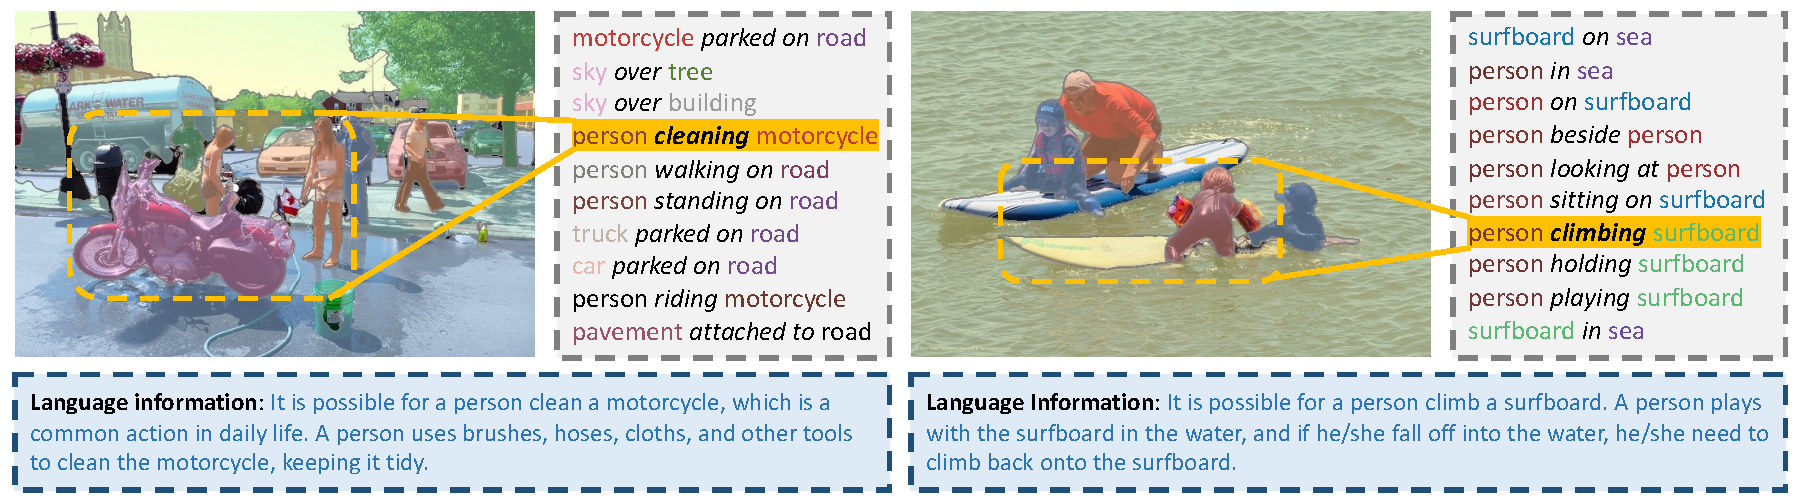
\includegraphics[width=1.0\linewidth]{Chapter4/Figures/vis_v1.pdf}
    \vspace{-4mm}
    \caption{Visualization results of our VLPrompt.
    We show two examples.
    For each example, the top left displays the predicted segmentation results, the top right shows the top 10 predicted relation triplets (all are correct relation triplets), and bottom is the language snippet utilized for predicting the highlighted triplets in yellow.
    }
    \vspace{-4mm}
    \label{vlprompt:fig:vis}
\end{figure}



\noindent \textbf{Failure case analysis.}
In addition to the high-quality visual results shown above, we also conduct a detailed failure case analysis, as illustrated in Fig.~\ref{vlprompt:fig:failure_vis}.
We observe that when multiple objects of the same category appear in close proximity within a scene, the model tends to mispredict the relations between them.
For example, in the first image from the left, 0\_person is only \textit{wearing} 3\_baseball\_glove, but the model incorrectly predicts that they are also \textit{wearing} 2\_baseball\_glove.
A similar misprediction occurs for 1\_person.
In the second image, only 0\_person is actually \textit{flying} the kite, while 1\_person and 2\_person are merely \textit{looking at} it.
When similar objects are located too close together, the segmentation model may mistakenly identify them as a single instance.
For example, in the fourth image, the model predicts that both 0\_person and 1\_person are \textit{riding} 2\_horse, whereas 2\_horse should be segmented into two separate horses instead of one.
Although incorporating language knowledge extracted from LLMs significantly alleviates the long-tail problem, reasoning about fine-grained relations between spatially adjacent objects remains a challenging issue that requires further investigation.


\noindent \textbf{Alleviating the long-tail problem.}
In SGG and PSG tasks, mR@K is often used as a reflection for a method's ability to solve long-tail problem~\citep{tang2020unbiased}.
To further validate it, in PSG dataset, we split relations occurring over 1000 times as common relations, and those under 1000 as rare relations, resulting into 21 common and 35 rare relations.
As shown in Tab.~\ref{vlprompt:tab:long_tail_psg}, our method's integration of language information (w/ LLM) leads to 2.3 increase in mR@100 for common relations and 13.8 increase for rare relations on the PSG dataset.
Tab.~\ref{vlprompt:tab:long_tail_vg} reveals consistent findings on the VG dataset.
The significant improvement in the latter highlights the effectiveness in enhancing rare relation prediction.
Additionally, as shown in Fig.~\ref{vlprompt:fig:predicate_wise}, we present relation/predicate-wise performance improvements on PSG dataset, further highlighting the effectiveness of our method across different relations.
Note, w/o LLM is our method without language information (Sec.~\ref{vlprompt:sec:method}).
In this setting, we remove the cross-attention module and rely solely on vision features for relation prediction.

\begin{table}[!t]
    \centering
    \setlength{\tabcolsep}{2.0mm}
    \caption{Alleviating the long-tail problem on PSG dataset.
    Incorporating LLM-based language information boosts performance on common and rare relations, with greater gains for rare ones, validating its effectiveness in addressing the long-tail problem.}
    % \resizebox{1.0\linewidth}{!}{
    \begin{tabular}{l|cccc}
    \toprule[1.3pt]
    ~ & \multicolumn{2}{c}{Common relations} & \multicolumn{2}{c}{Rare relations}\\
    ~ & w/o LLM & w/ LLM & w/o LLM & w/ LLM\\
    \midrule
    mR@100 & 54.7 & \textbf{57.0 (\textcolor{darkgreen}{+2.3})} & 37.9 & \textbf{51.7 (\textcolor{darkgreen}{+13.8})} \\
    \bottomrule[1.3pt]
    \end{tabular}
    % }
    \label{vlprompt:tab:long_tail_psg}
\end{table}


\begin{table}[!t]
    \centering
    \setlength{\tabcolsep}{2.0mm}
    \caption{Alleviating the long-tail problem on VG dataset.}
    % \resizebox{1.0\linewidth}{!}{
    \begin{tabular}{l|cccc}
    \toprule[1.3pt]
    ~ & \multicolumn{2}{c}{Common relations} & \multicolumn{2}{c}{Rare relations}\\
    ~ & w/o LLM & w/ LLM & w/o LLM & w/ LLM\\
    \midrule
    mR@100 & 21.6 & \textbf{23.2 (\textcolor{darkgreen}{+1.6})} & 9.7 & \textbf{16.4 (\textcolor{darkgreen}{+6.7})} \\
    \bottomrule[1.3pt]
    \end{tabular}
    % }
    \label{vlprompt:tab:long_tail_vg}
\end{table}



\begin{figure}[H]
    \centering
    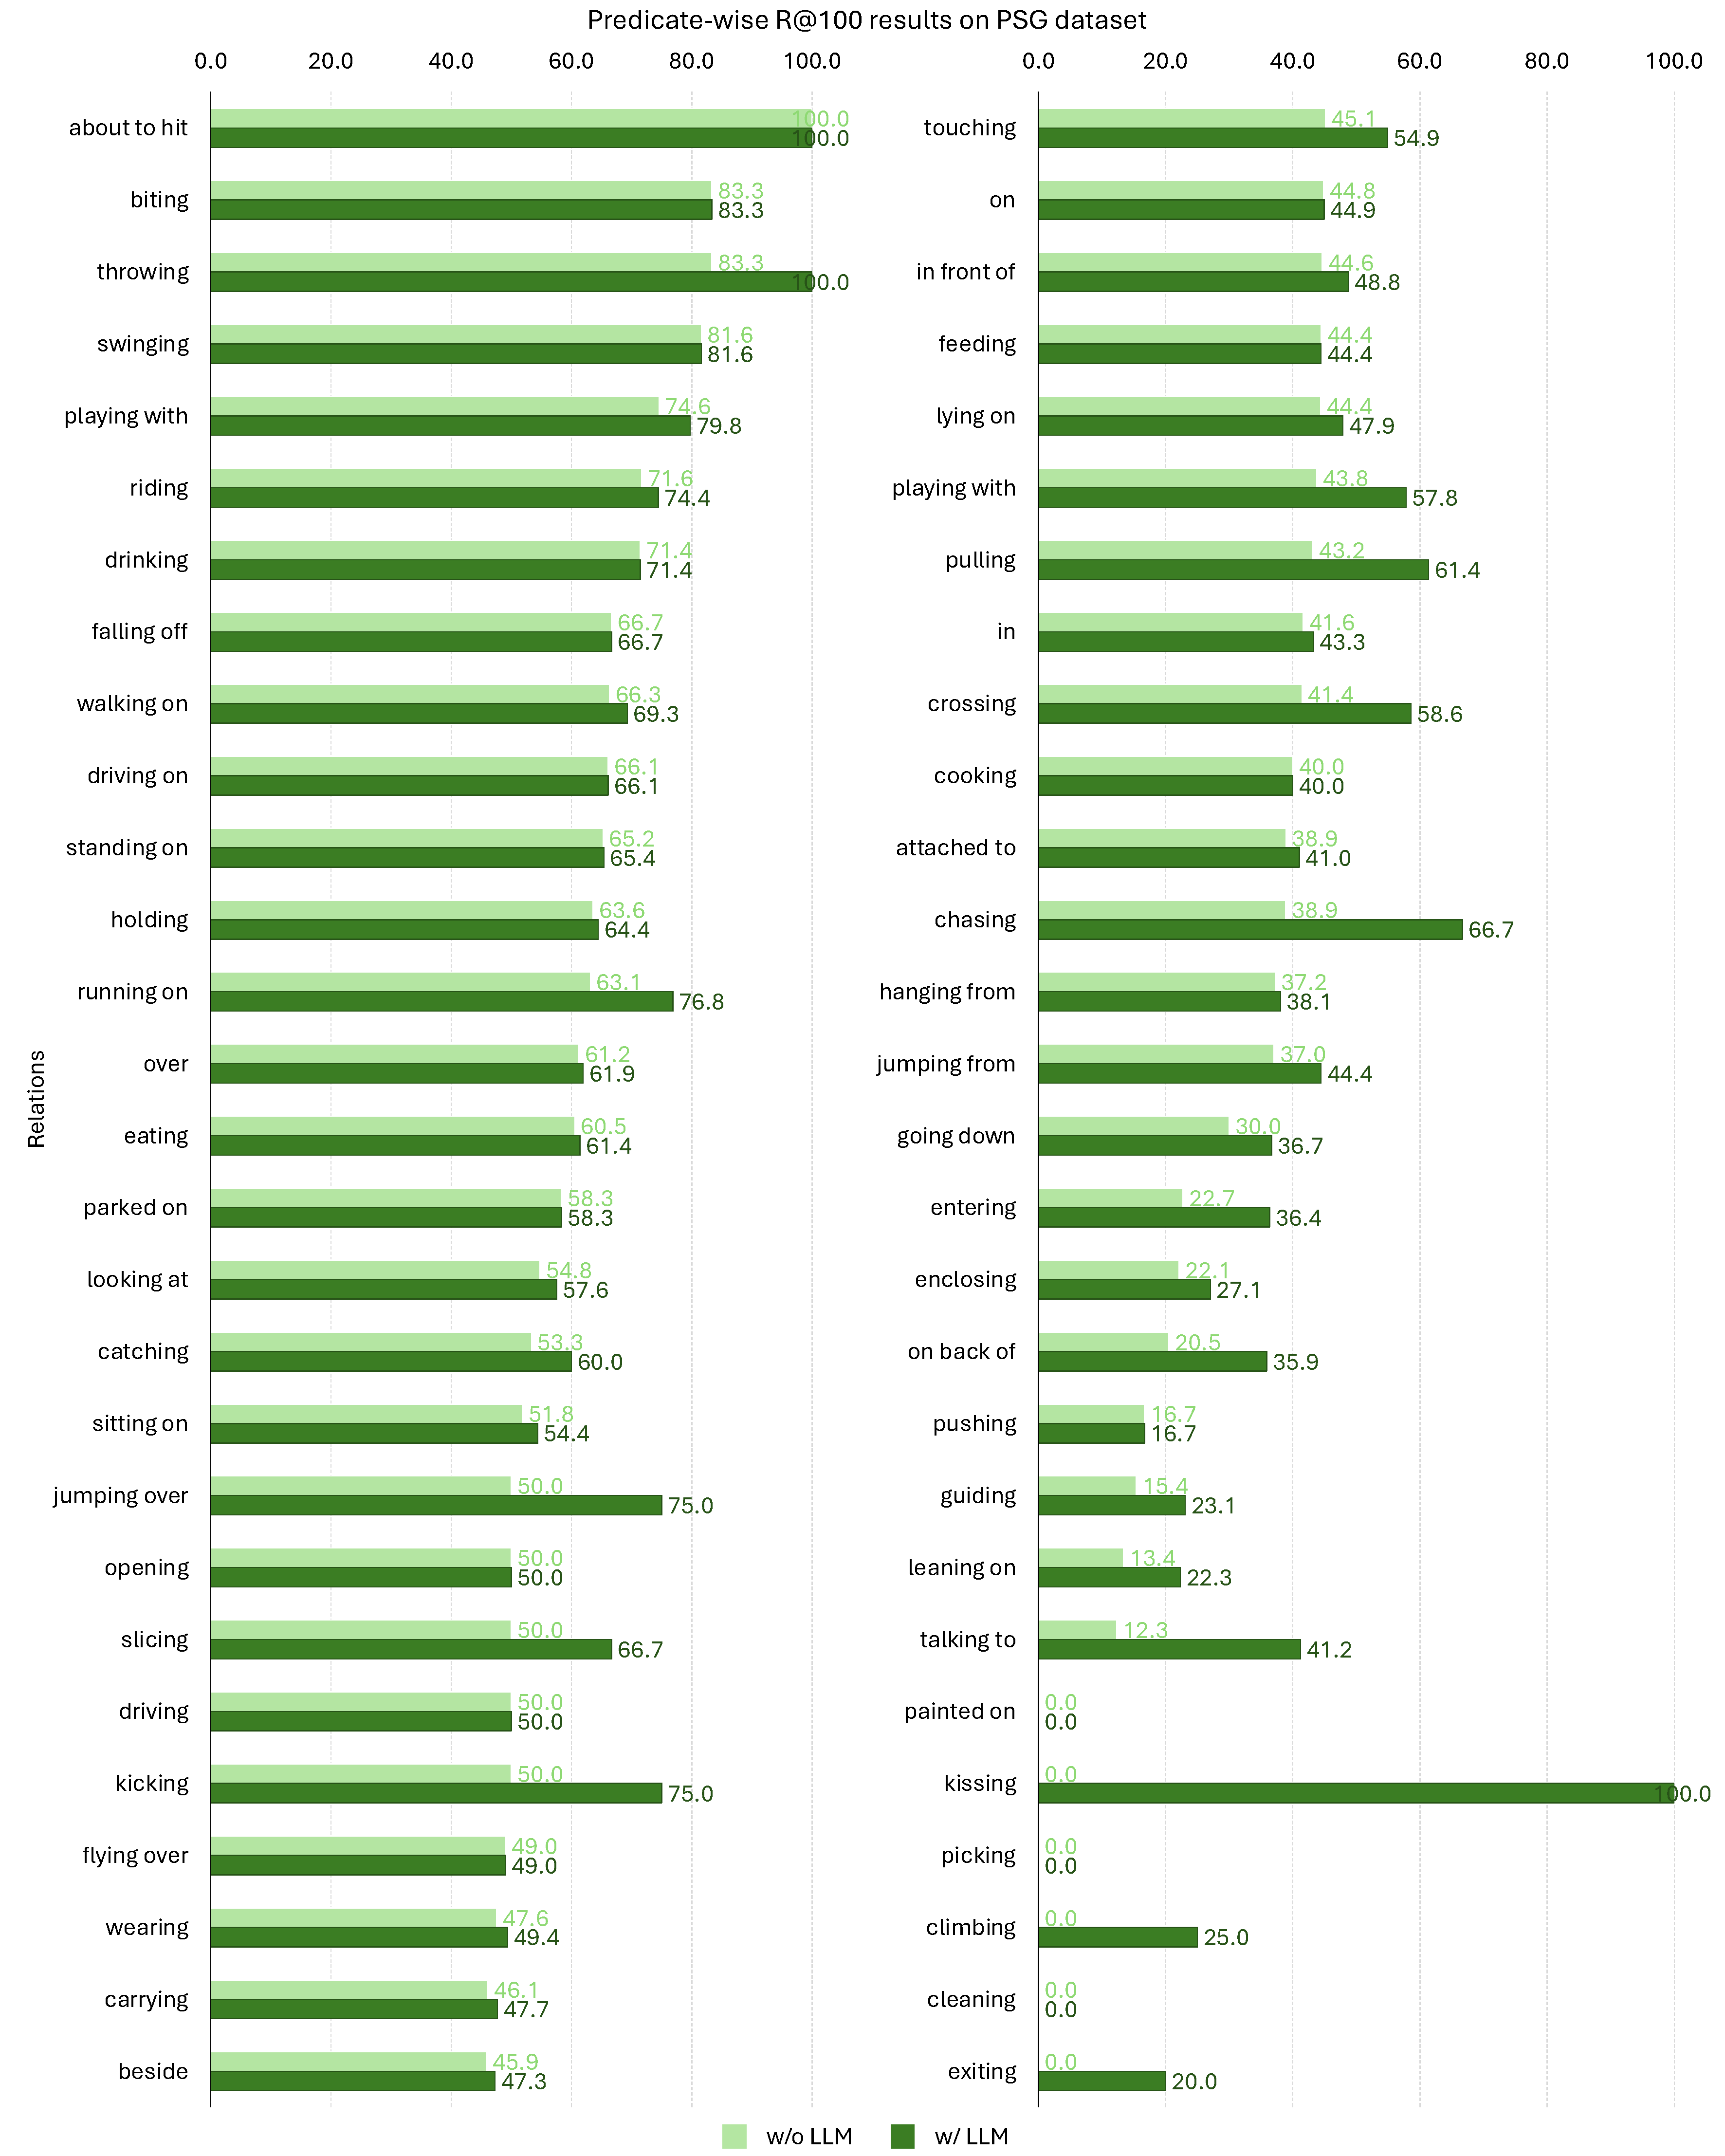
\includegraphics[width=1.05\linewidth]{Chapter4/Figures/predicate_wise_v2.pdf}
    \vspace{-2mm}
    \caption{Predicate-wise R@100 results on the PSG dataset show performance improvements across various relations with LLM integration.}
    \label{vlprompt:fig:predicate_wise}
\end{figure}



\begin{figure}[!t]
    \centering
    \begin{subfigure}{0.5\textwidth}
        \centering
        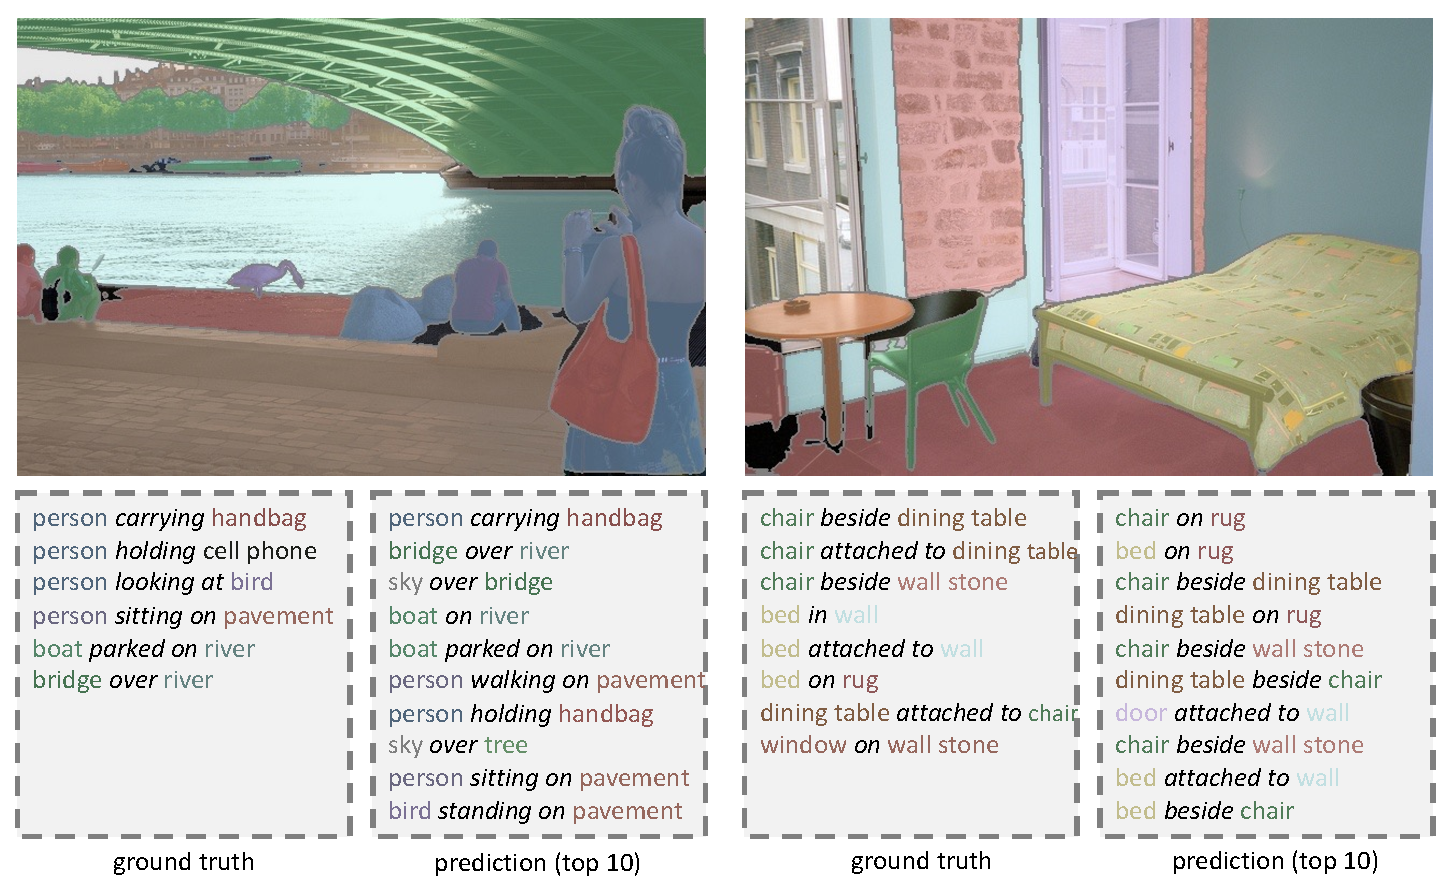
\includegraphics[width=\linewidth]{Chapter4/Figures/vis_v3.pdf}
    \end{subfigure}
    \hspace{-2mm}
    \begin{subfigure}{0.5\textwidth}
        \centering
        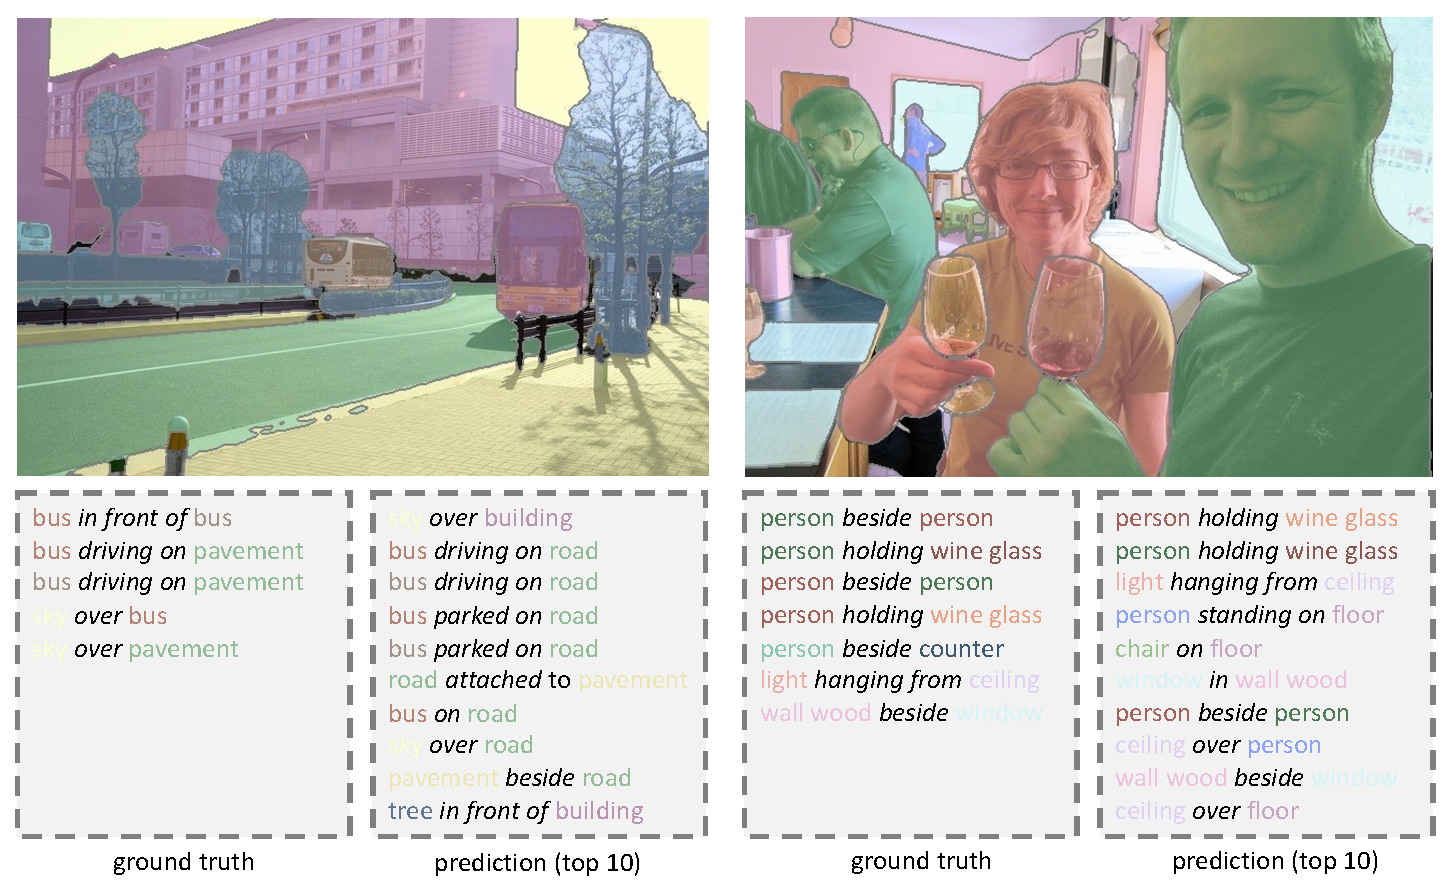
\includegraphics[width=\linewidth]{Chapter4/Figures/vis_v4.pdf}
    \end{subfigure}
    \begin{subfigure}{0.5\textwidth}
        \centering
        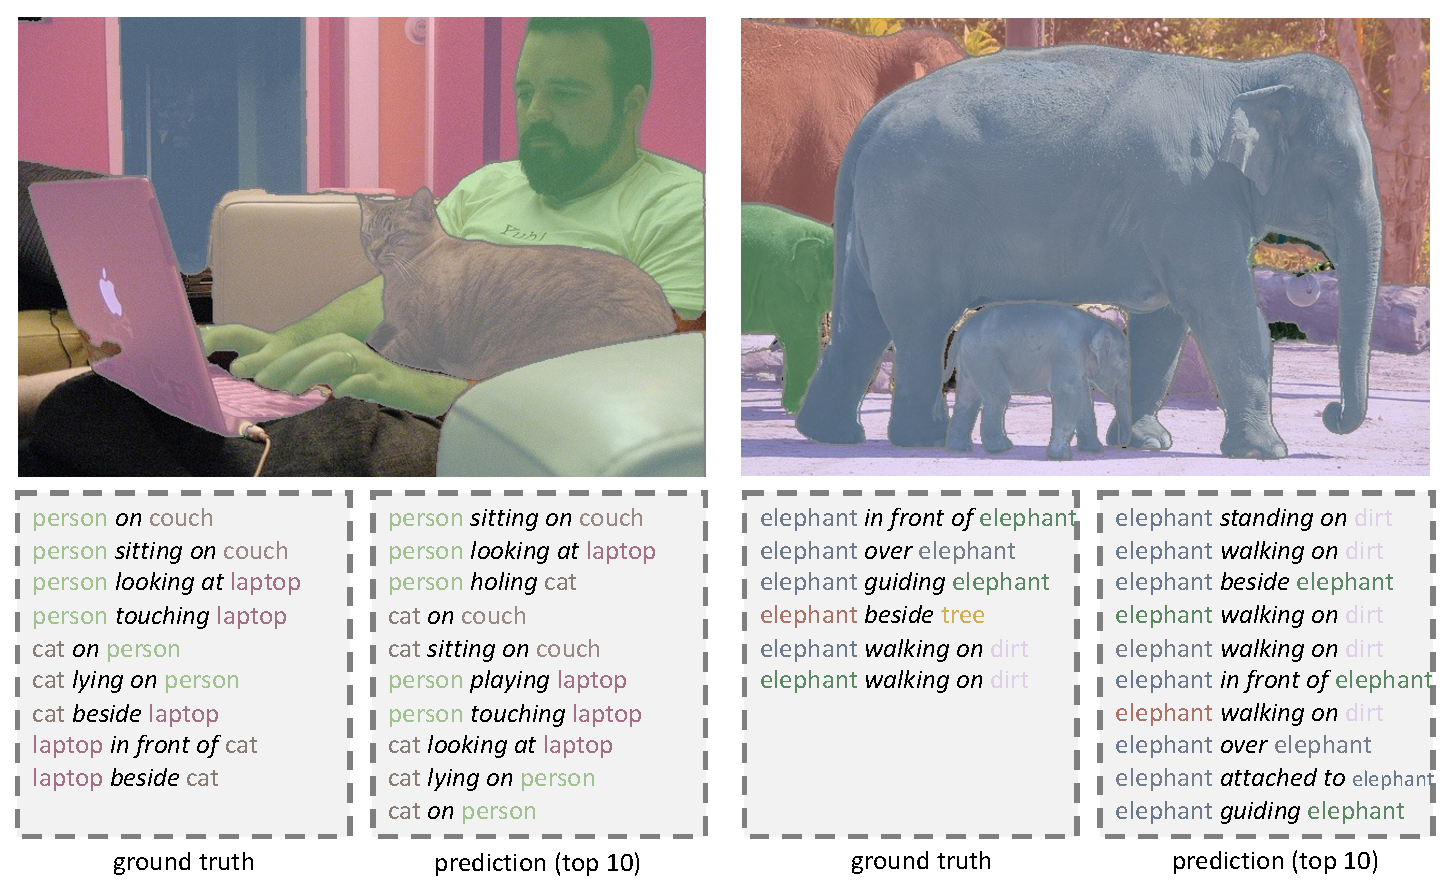
\includegraphics[width=\linewidth]{Chapter4/Figures/vis_v6.pdf}
    \end{subfigure}
    \hspace{-2mm}
    \begin{subfigure}{0.5\textwidth}
        \centering
        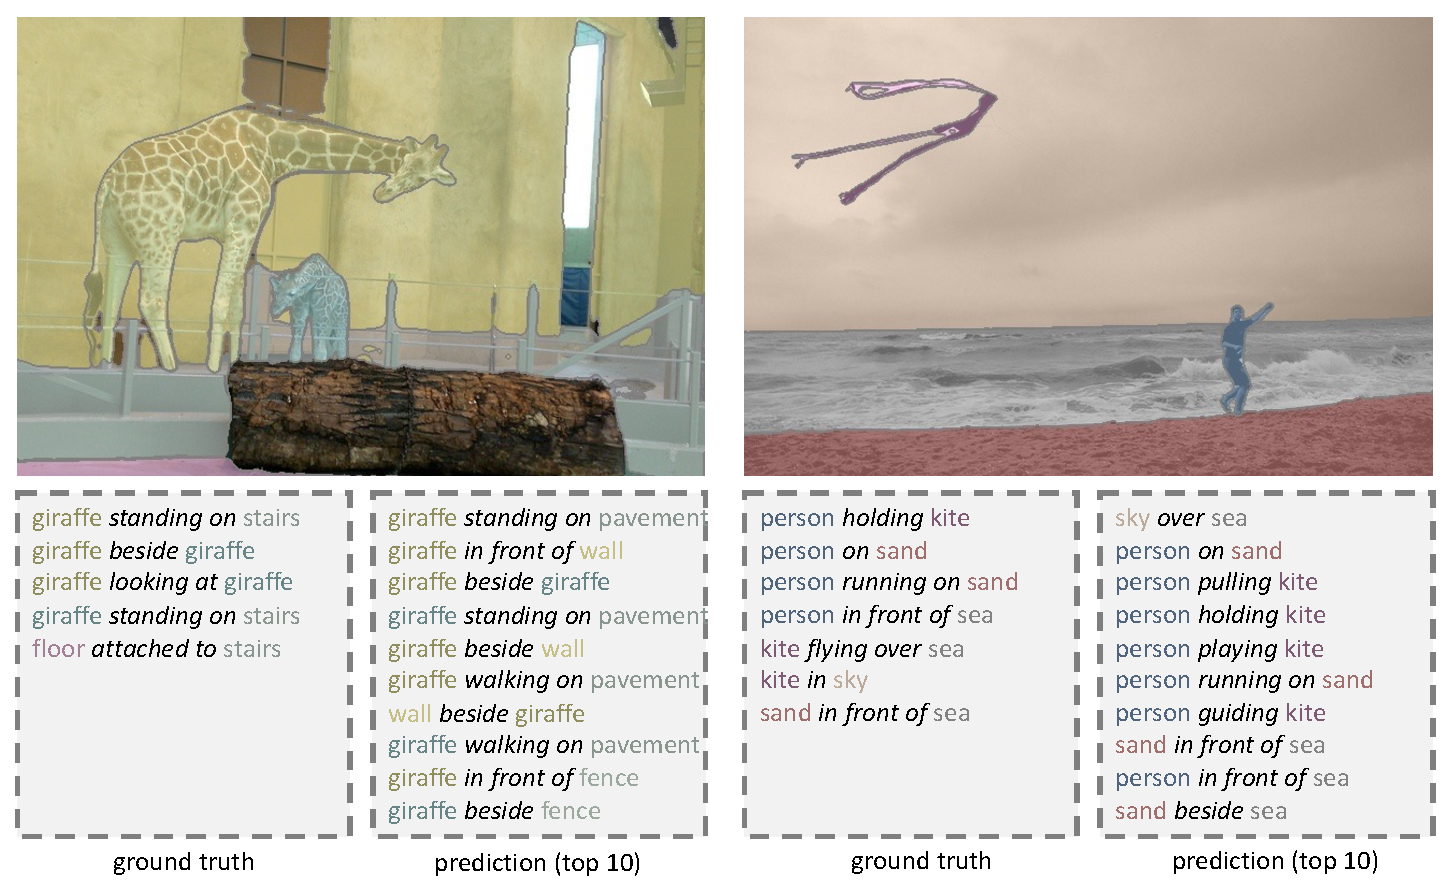
\includegraphics[width=\linewidth]{Chapter4/Figures/vis_v7.pdf}
    \end{subfigure}
    \caption{Visualization of panoptic segmentation (top), ground truth (bottom left), and top 10 relation predictions (bottom right) demonstrates VLPrompt's precision in relation prediction, enhancing scene understanding.}
    \label{vlprompt:fig:more_vis}
    \vspace{-6mm}
\end{figure}



\begin{figure}[!t]
    \centering
    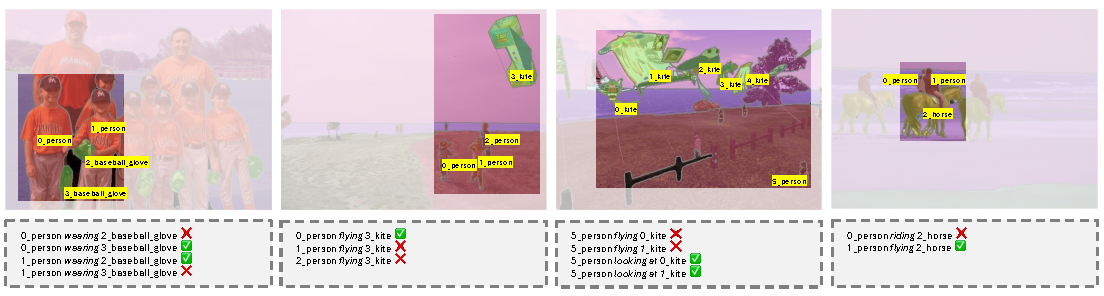
\includegraphics[width=1.0\linewidth]{Chapter4/Figures/failure_case_analysis_v2.pdf}
    \vspace{-4mm}
    \caption{Visualization of typical failure cases.
    We visualize typical failure cases of VLPrompt, which mainly occur when multiple instances of the same object category appear in the scene.
    In such cases, the model often mismatches the relations between different objects.
    }
    \vspace{-4mm}
    \label{vlprompt:fig:failure_vis}
\end{figure}



\noindent \textbf{Comparison with large multimodal models.}
Large multimodal models (LMMs) currently demonstrate great performance across various multimodal tasks and can also predict relations with specific instructions.
To further validate the performance of LMMs on PSG task, we test three popular LMMs GPT-4o, GPT-4V and Llama 3.2-11B on the PSG test set.
To ensure fairness in comparison, we allow LMMs to use the segmentation results output by our method, thus ensuring same segmentation performance.
Specifically, following the approach of \citet{yang2023setofmark}, we attach the panoptic segmentation results extracted by our model to the original image and input it to LMMs.
This allows LMMs to obtain object segmentation results and the corresponding categories consistent with our method.
Subsequently, we use LMMs to predict the relations for all object pairs.
From the experimental results, as shown in Tab.~\ref{vlprompt:tab:gpt_4v}, we observe that as more advanced LMMs are used, their performance steadily improves.
However, a noticeable performance gap still remains compared to our PSG model.
This trend indicates that LMMs hold strong potential for achieving better results.
In turn, we believe that future advances in LMMs may further promote progress in panoptic scene graph generation.

\begin{table}[!t]
    \centering
    \setlength{\tabcolsep}{1.2mm}
    \caption{Comparison with LMMs in PSG task.
    Large multimodal models like GPT-4V, not tailored for PSG task, underperform compared to task-specific PSG models.}
    % \resizebox{1.0\linewidth}{!}{
    \begin{tabular}{l|cccccc}
    \toprule[1.3pt]
    Method & R@20 & mR@20 & R@50 & mR@50 & R@100 & mR@100 \\
    \midrule
    VLPrompt & \textbf{39.4} & \textbf{34.7} & \textbf{47.6} & \textbf{45.1} & \textbf{52.4} & \textbf{53.7} \\
    GPT-4o~\citep{chatgpt} & 30.9 & 28.6 & 40.2 & 38.9 & 45.9 & 44.1 \\
    GPT-4V~\citep{chatgpt} & 16.9 & 10.1 & 20.4 & 12.8 & 22.5 & 13.1 \\
    Llama 3.2-11B~\citep{dubey2024llama} & 14.8 & 6.9 & 16.9 & 8.2 & 18.1 & 9.5 \\
    \bottomrule[1.3pt]
    \end{tabular}
    % }
    \label{vlprompt:tab:gpt_4v}
\end{table}


\subsection{Ablation study}

\subsubsection{Vision Feature Extractor}

\begin{table}[!t]
    \centering
    \setlength{\tabcolsep}{1.2mm}
    \caption{Ablation study for the Vision Feature Extractor.}
    % \resizebox{1.0\linewidth}{!}{
    \begin{tabular}{l|cccccc}
    \toprule[1.3pt]
    Method & R@20 & mR@20 & R@50 & mR@50 & R@100 & mR@100 \\
    \midrule
    VLPrompt & \textbf{39.4} & \textbf{34.7} & \textbf{47.6} & \textbf{45.1} & \textbf{52.4} & \textbf{53.7} \\
    ~~~~PixelDec $\rightarrow$ TsfmDec & 37.4 & 32.1 & 45.8 & 43.7 & 50.1 & 50.3 \\
    ~~~~MaskPool $\rightarrow$ BboxPool & 38.6 & 33.7 & 46.4 & 44.8 & 51.0 & 52.6 \\
    ~~~~Concat. $\rightarrow$ Sub. & 35.4 & 29.8 & 44.1 & 42.3 & 48.6 & 48.9 \\
    ~~~~w/o Spatial Feat. & 39.0 & 33.0 & 46.6 & 44.3 & 51.7 & 52.1 \\
    \bottomrule[1.3pt]
    \end{tabular}
    % }
    \label{vlprompt:tab:ablation_vision_feature_extractor}
\end{table}

\noindent \textbf{Object features from pixel decoder.}
To validate the superiority of obtaining object features from the pixel decoder (PixelDec) of Mask2Former, we experiment with an alternative approach: acquiring corresponding object features from the transformer decoder (TsfmDec) of Mask2Former. This is a common practice in the literature~\citep{cong2023reltr}.
Experiments (PixelDec$\rightarrow$TsfmDec) in Tab.~\ref{vlprompt:tab:ablation_vision_feature_extractor} show that the feature from the pixel decoder performs 3.4 better in mR@100 than that from the transformer decoder, as the pixel decoder contains more comprehensive vision information.

\noindent \textbf{Mask pooling for object feature extraction.}
Common methods to obtain object features from the pixel decoder include mask pooling (MaskPool) and bounding box pooling (BboxPool)~\citep{girshick2015fast}.
We validate our choice of mask pooling through ablation experiments (MaskPool$\rightarrow$BboxPool).
As shown in Tab.~\ref{vlprompt:tab:ablation_vision_feature_extractor}, the performance using mask pooling is 1.1 higher in mR@100 than that using bbox pooling.
Mask pooling is more suitable for the mask prediction in the PSG task. 

\noindent \textbf{Concatenating object features into a pair feature.}
Common methods for merging the features of two objects for their relation prediction include concatenation (Concat.) \citep{zhang2019graphical} and subtraction (Sub.) \citep{cheng2022visual}.
Notably, addition of the features cannot be used due to the inherent order requested between the subject and object.
Results (Concat.$\rightarrow$Sub.) in Tab.~\ref{vlprompt:tab:ablation_vision_feature_extractor} indicate that concatenation outperforms subtraction by 4.8 on the mR@100.

\noindent \textbf{Spatial feature.}
To validate the effect of adding spatial features, we conduct an ablation study by removing these features.
The results (w/o Spatial Feat.) in Tab.~\ref{vlprompt:tab:ablation_vision_feature_extractor} show that this leads to a decrease of -0.7 in R@100 and -1.6 in mR@100.
This is because spatial features provide the model with additional spatial interaction between the subject and object (Sec.~\ref{vlprompt:sec:vision_feature_extractor}), thereby enhancing the vision feature for relation prediction.


\subsubsection{Language Feature Extractor}

\begin{table}[!t]
    \centering
    \setlength{\tabcolsep}{1.2mm}
    \caption{Ablation study for the Language Feature Extractor.}
    % \resizebox{1.0\linewidth}{!}{
    \begin{tabular}{l|cccccc}
    \toprule[1.3pt]
    Method & R@20 & mR@20 & R@50 & mR@50 & R@100 & mR@100 \\
    \midrule
    VLPrompt & \textbf{39.4} & \textbf{34.7} & \textbf{47.6} & \textbf{45.1} & \textbf{52.4} & \textbf{53.7} \\
    ~~~~w/o CoT & 36.8 & 27.9 & 44.3 & 38.8 & 48.6 & 45.7 \\
    ~~~~w/o template & 39.0 & 33.7 & 47.0 & 43.8 & 51.6 & 52.2 \\
    ~~~~Ext$^\text{RP} \rightarrow$ Ext$^\text{RJ}$ & 39.1 & 34.2 & 47.5 & 45.1 & 52.3 & 53.5 \\
    ~~~~Ext$^\text{RJ} \rightarrow$ Ext$^\text{RP}$ & 38.9 & 31.2 & 46.8 & 41.7 & 51.0 & 49.9 \\
    ~~~~Swap(Ext$^\text{RP}$, Ext$^\text{RJ}$)~~~~ & 36.2 & 29.4 & 44.3 & 38.6 & 48.7 & 46.4 \\
    ~~~~Llama3-8B + Bert & 39.0 & 33.5 & 47.3 & 44.8 & 52.0 & 53.2 \\
    ~~~~Compression & 38.3 & 33.1 & 46.5 & 44.6 & 51.2 & 51.1 \\
    \bottomrule[1.3pt]
    \end{tabular}
    % }
    \label{vlprompt:tab:ablation_language_feature_extractor}
\end{table}

\noindent \textbf{Chain-of-thought for prompt.}
By carefully designing prompts with the chain-of-thought technique, LLMs can produce rich and accurate descriptions.
However, if we do not use chain-of-thought and instead directly ask LLMs questions, such as replacing the relation proposer prompt with ``What are the possible relations between subject and object? And why?'' or the relation judger prompt with ``Could this relation be possible between subject and object? Why?", we find that the outputs from LLMs become much less predictable and often not as expected.
We experiment without chain-of-thought (w/o CoT) and the results in Tab.~\ref{vlprompt:tab:ablation_language_feature_extractor} show that the performance of relation prediction significantly drops, \ie, a -8.0 decrease in mR@100.
This further illustrates the rationale and importance of using chain-of-thought technology for designing prompts.

\noindent \textbf{Template phrase in RP-prompt.}
The template phrase appended to the end of the RP-prompt helps the model clearly distinguish common relations from less plausible ones, thereby preventing performance degradation on high-frequency relations during prediction.
To validate this design, we conduct an ablation study by removing the template phrase.
As shown in Tab.~\ref{vlprompt:tab:ablation_language_feature_extractor} (w/o template), excluding the template leads to a slight performance drop ($-0.8$ R@100, $-1.5$ mR@100), indicating that explicitly guiding the model to differentiate between common and uncommon relations through prompt design is beneficial.

\noindent \textbf{Different feature extraction methods.}
To validate our design of different feature extract methods for RP- and RJ-language prompting features, we study their effects.
We offer three variants:
1) For RP-language prompting features, we adopt the same way as the RJ-language prompting feature to extract feature for each relation triplet individually, we denote this variant as Ext$^\text{RP} \rightarrow$ Ext$^\text{RJ}$ in the Tab.~\ref{vlprompt:tab:ablation_language_feature_extractor}.
It shows that performance is slightly lower than our original VLPrompt, but with increased computation.
2) For RJ-language prompting features, we adopt the same way as the RP-language prompting feature to extract all relation triplets into one feature, denoted by Ext$^\text{RJ} \rightarrow$ Ext$^\text{RP}$ in the Tab.~\ref{vlprompt:tab:ablation_language_feature_extractor}.
We observe a clear drop in mR@K, as this would condense the features of relations between subject and object while dropping the subtle details, which can be especially disadvantageous for rare relations.
3) We swap the feature extraction methods between Ext$^\text{RP}$ and Ext$^\text{RJ}$, denoted by Swap(Ext$^\text{RP}$, Ext$^\text{RJ}$) in Tab.~\ref{vlprompt:tab:ablation_language_feature_extractor}.
We observe a substantial decrease in both metrics.
Our original feature extraction is specifically designed on one side to focus on the condensed and distinct attributes of commonly occurring relations; on the other side to focus on the detailed and subtle attributes of all possible especially rare relations for a subject-object pair.

\noindent \textbf{Different LLMs and text encoders.}
To further assess the effects of different LLMs and text encoders on model performance, we attempt to replace the GPT-4 with Llama3-8B~\citep{touvron2023llama} and the OpenAI Embedding Service with Bert~\citep{devlin2018bert}.
When using Bert, we take the mean of the embeddings of all output tokens as the feature.
The experimental results (Llama3-8B + Bert) in Tab.~\ref{vlprompt:tab:ablation_language_feature_extractor} reveal that using Llama3-8B as the LLM and Bert as the text encoder results in only a slight decrease in performance: -0.4 in R@100 and -0.5 in mR@100.
We review the descriptions output by Llama3-8B and compare them with those from GPT-4, finding no significant differences in quality, more details can be found in supplementary materials.
This suggests that, with carefully designed prompts, open-source LLMs with reduced parameters also work for our method, thus validating the flexibility of our method.

\noindent \textbf{Compress the language prompting feature.}
At runtime, the language prompting feature occupies 290.57MB of memory, which is manageable.
To further enhance the model's applicability in real-world scenarios, such as when there are more object and relation categories, we compress the language prompting feature to 1/4 of its original size using an encoder-decoder models.
Results (Compression) shown in Tab.~\ref{vlprompt:tab:ablation_language_feature_extractor} indicate that compressing the language prompting feature to 1/4 leads to only a minor performance decrease, while the memory required by the model during runtime is reduced to 1/4 of the original, which further demonstrates the practicality of our method in real-world settings.



\subsubsection{Vision-Language Prompter}

\begin{table}[!t]
    \centering
    \setlength{\tabcolsep}{1.2mm}
    \caption{Ablation study for the Vision-Language Prompter.}
    % \resizebox{1.0\linewidth}{!}{
    \begin{tabular}{l|cccccc}
    \toprule[1.3pt]
    Method & R@20 & mR@20 & R@50 & mR@50 & R@100 & mR@100 \\
    \midrule
    VLPrompt & \textbf{39.4} & \textbf{34.7} & \textbf{47.6} & \textbf{45.1} & \textbf{52.4} & \textbf{53.7} \\
    ~~~~w/o Language~~~~~~ & 37.1 & 26.8 & 45.9 & 37.2 & 50.0 & 44.2 \\
    ~~~~RP-decoder & 38.4 & 30.6 & 46.6 & 41.2 & 50.9 & 49.6 \\
    ~~~~RJ-decoder & 37.9 & 34.2 & 45.3 & 44.6 & 50.4 & 52.8 \\
    ~~~~Uncompressed $F_L^{RJ}$ for $W^{RJ}$ & 39.3 & 34.7 & 47.5 & 44.9 & 52.1 & 53.7 \\
    \bottomrule[1.3pt]
    \end{tabular}
    % }
    \label{vlprompt:tab:ablation_vision_language_prompter}
    \vspace{-2mm}
\end{table}

\noindent \textbf{Language information.}
To validate the efficacy of incorporating language information, we conduct a comparative experiment by replacing all language prompting features in the vision-language prompter with vision prompting features.
This approach ensures that all other factors remain constant while assessing the impact of language information.
As shown in Tab.~\ref{vlprompt:tab:ablation_vision_language_prompter}, the experimental results (w/o Language) reveal a significant decrease in the mR@100 by -9.5 when language information is removed, which demonstrates the substantial impact of language information in mitigating the long-tail problem.

\noindent \textbf{Results of RP-decoder and RJ-decoder.}
We test the relation prediction performance of both RP-decoder and RJ-decoder separately.
The results (RP-decoder and RJ-decoder) in Tab.~\ref{vlprompt:tab:ablation_vision_language_prompter} show that the RP-decoder outperforms the RJ-decoder in the R@K (\eg, 50.9 \vs 50.4 for R@100), while the RP-decoder scores lower in mR@K compared to the RJ-decoder (\eg, 49.6 \vs 52.8 for mR@100).
This indicates that the RP-decoder is good at predicting frequent relation classes, whereas the RJ-decoder excels in rare relation classes, which indicates that they are complementary.

\noindent \textbf{Relation fusion.}
As shown in Tab.~\ref{vlprompt:tab:ablation_vision_language_prompter}, when the outputs of the two branches are combined via our relation fusion strategy (\ie, VLPrompt), the final prediction outperforms either individual branch, demonstrating the effectiveness of our design.
Specifically, the RP-decoder achieves higher R@K but lower mR@K scores compared to the RJ-decoder, as it receives RP-language prompting features that encode the most frequent relations for each subject-object pair.
This makes the model more biased toward high-frequency relations, resulting in strong performance on common categories but poor generalization to rare ones, due to the long-tail distribution of relation labels.
In contrast, the RJ-decoder, which uses RJ-language prompting features to independently judge each relation category, achieves better mR@K at the cost of slightly reduced R@K, as it improves rare-relation prediction by sacrificing some performance on frequent ones.
These complementary behaviors highlight the importance of integrating both decoders, allowing the model to leverage their respective strengths and achieve overall optimal performance.

\noindent \textbf{Fusion weights.}
The input feature $F_L^{RJ}$ used to compute the fusion weights $W^{RJ}$ is compressed along the relation dimension, and this operation is applied solely within the gate network.
Our empirical results show that this compression has minimal impact on performance, as the gate network is only responsible for generating fusion weights.
To validate this design choice, we conduct an ablation study.
As shown in Tab.~\ref{vlprompt:tab:ablation_vision_language_prompter} (Uncompressed $F_L^{RJ}$ for $W^{RJ}$), using the uncompressed $F_L^{RJ}$ yields performance comparable to its compressed counterpart.
This confirms that the compressed version of $F_L^{RJ}$ offers a more computationally efficient implementation without sacrificing performance.



\begin{table}[!t]
    \centering
    \setlength{\tabcolsep}{1.2mm}
    \caption{Ablation study for the number of decoder blocks.}
    % \resizebox{1.0\linewidth}{!}{
    \begin{tabular}{c|cccccc}
    \toprule[1.3pt]
    ~~~~~Block Number~~~~~ & R@20 & mR@20 & R@50 & mR@50 & R@100 & mR@100 \\
    \midrule
    1 & 35.1 & 29.8 & 44.8 & 39.5 & 47.2 & 46.9 \\
    2 & \textbf{39.4} & 34.7 & \textbf{47.6} & 45.1 & \textbf{52.4} & 53.7 \\
    4 & 38.9 & \textbf{34.8} & 47.4 & \textbf{45.2} & 52.1 & \textbf{53.9} \\
    12 & 18.4 & 14.5 & 27.5 & 23.0 & 33.2 & 29.4 \\
    \bottomrule[1.3pt]
    \end{tabular}
    % }
    \label{vlprompt:tab:ablation_decoder_block_number}
\end{table}

\noindent \textbf{The number of decoder blocks.}
To elucidate the reason that both RP-decoder and RJ-decoder use a 2-block transformer decoder, we vary different numbers of blocks in Tab.~\ref{vlprompt:tab:ablation_decoder_block_number}.
We observe that when increasing the transformer decoder blocks from 1 to 2, there is a significant improvement in model performance.
However, increasing from 2 to 4 blocks does not change much for the performance.
Further increasing the decoder blocks to 12 leads to a notable decrease in performance, suggesting that too many decoder blocks may cause the model to overfit.
Considering both performance and speed, we choose 2 blocks.


\subsubsection{Efficiency Analysis}

\begin{table}[!t]
    \centering
    \caption{Analysis for efficiency.
    Our method achieves significant performance improvements without introducing notable efficiency issues, maintaining a comparable level to previous approaches.
    }
    % \resizebox{0.8\linewidth}{!}{
    \begin{tabular}{l|ccc}
    \toprule[1.3pt]
    Method & FLOPS (G) & Parameters (G) & Inference Speed (ms) \\
    \midrule
    PSGTR \citep{yang2022panoptic} & 461.3 & 44.2 & 140 \\
    HiLo \citep{zhou2023hilo} & 229.4 & 58.7 & 156 \\
    VLPrompt (ours) & 386.7 & 49.1 & 152 \\
    \bottomrule[1.3pt]
    \end{tabular}
    % }
    \label{vlprompt:tab:analysis_efficiency}
\end{table}

In Tab.~\ref{vlprompt:tab:analysis_efficiency}, we compare our model's efficiency with the previous state-of-the-art models, evaluating computational floating point operations per second (FLOPS), parameter size and inference speed on the same A100 GPU.
We observe that although our method has higher FLOPS compared to HiLo, it matches HiLo in prediction speed, and significantly outperforms HiLo in performance (see Tab.~\ref{vlprompt:tab:psg_results}).
